\chapter{Related work}
\label{sec:related_work}

This section is subdivided into two parts. First, publications discussing \textit{mesh saliency}, a technique used term to predict regional percieved importance of digital representations of real-world (or synthetic) objects as well as 2D images, will be presented and briefly described. The second section will provide a look into human behavior, based on cognition and outside stimuli in virtual reality environments. These two sets of scientific works will provide a solid knowledge of terms and methods commonly used in this field and describe the current state of the art.

\section{Mesh saliency and human perception}
\label{sec:mesh_saliency_and_human_perception}

Research on what human perception guides us to focus our attention on when presented with an 3D representation of an object was begun just past the year 2000 and has been a continuous effort ever since. One commonly cited publication in this field is Lee \textit{et al.} \cite{lee2005mesh}. Based on low-level human visual attention \cite{koch1987shifts}, it introduces the term \textit{mesh saliency}, a measure for regional based importance of 3D meshes, and also presents a way to compute it. This fully automatic process successfully predicts  what would be classified by most observers as prominent, visually interesting regions on a mesh, thus allowing mesh operations such as simplification \cite{cignoni1998comparison} and segmentation \cite{shamir2008survey} to produce results that are more appealing to the beholder.

\begin{figure}[htb]
  \centering
  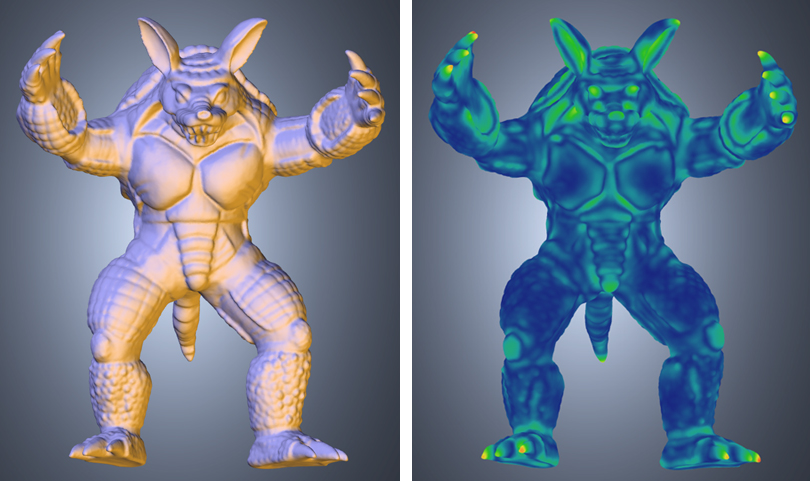
\includegraphics[width=1.0\textwidth]{arma.png}\\ % PNG-File
  \caption{A model and its computes mesh saliency map. Published by Lee \textit{et al.} \cite{lee2005mesh}. Bright colors (yellow and red) indicate high saliency values for their respective vertices, dark colors (shades of blue) indicate low values.}\label{fig:lee_arma_map}
\end{figure}

The model for computing \textit{mesh saliency} is based on a center-surround comparison of local curvature. It is scale-dependent on a \textit{saliency factor} $\varepsilon$, which is based on the diagonal of the objects bounding box, and is able to identify salient features of a mesh, depending on their surrounding area. Geometrically complex regions, for example a large patch containing lots of bumps of similar size, will be rightfully dismissed as, in most cases, regions that are not interesting from a human perceptional stance.

Taking a closer look at the basic formula through which saliency for any vertex of a mesh can be computed according to Lee \textit{et al.} helps understanding the underlying concept. As a first step, the mean curvature map for a mesh, describing mean local curvature values on a point-level for each of its vertices, needs to be calculated via commonly known approaches such as \cite{taubin1995estimating}. The resulting mean curvature map $\mathscr{C}$ defines a mapping from each vertex of a mesh to its mean curvature $\mathscr{C}$(\textit{v}). Using a distance measure such as the Euclidean or geodesic method, one can compute the neighbourhood \textit{N}(\textit{v},$\sigma$) of a vertex \textit{v} which then defines a set of points within a distance $\sigma$. The Euclidean appraoch was used in Lee \textit{et al.} and subsequently in the formula below.
Using these definitions, the authors denote the Gaussian-weighted average of the mean curvature by G($\mathscr{C}$(\textit{v}),$\sigma$) and present the following way of computing it.

\begin{align*}
G(\mathscr{C}(v),\sigma) &= \frac
	{
		\sum_{x \in N(v,2\sigma)}
			\mathscr{C}(x)exp	-||x-v||^2 \backslash(2\sigma^2)
	}{
		\sum_{x \in N(v,2\sigma)}
			exp -||x-v||^2 \backslash(2\sigma^2)
	}
\end{align*}

For computation of the Gaussian-weighted average, a cut-off factor for the filter is assumed at a distance of 2$\sigma$, in other words twice the distance that a vertex can have to another vertex to still be considered in its neighbourhood.
Based on these definitions, the saliency $\mathscr{S}$(\textit{v}) of a vertex \textit{v} is defined as the abslute difference between the Gaussian-weighted averages, as seen in the formula below.

\begin{align*}
\mathscr{S}(\textit{v}) &= |\textit{G}(\mathscr{C}(\textit{v}),\sigma) - G(\mathscr{C}(\textit{v}),2\sigma)|
\end{align*}

In order to get more refined results, one can conduct multiple computations of \textit{mesh saliency} with different values for $\sigma$. Lee \textit{et al.} use the previously mentioned \textit{saliency factor} $\varepsilon$ with $\varepsilon \in [2,6]$ in their paper, to generate multiple values for $\sigma$.

The concept of \textit{mesh saliency} has since been refined, augmented and adapted to serve as a basis for a multitude of specific use-cases and applications. When processing single vertex saliency, Wu \textit{et al.} \cite{wu2013mesh} took into consideration not only the curvature of the region surrounding the vertex, but also the global context of it. In other words, for each vertex to be attributed a value describing its saliency, its \textit{global rarity}, derived from comparing its features to those of every other vertex of the object, is computed. They performed a user study in which they had participants choose one out of two saliency maps for a set of objects, presented in a random order. One map was generated using their approach, the other one with the model presented in Lee \textit{et al.} Participants were asked to pick the one that was a closer representation of what they would have considered interesting regions and features. Since their method got picked in almost 58 per cent of cases, while the results produced by the model presented in Lee \textit{et al.} were favored in about 42 per cent, this can be considered a true improvement of the way \textit{mesh saliency} can be computed.

One approach to improve the method of finding salient elements in 2D images relied on paying extra attention to depth-information in \cite{ciptadi2013depth}. In this work, Ciptadi \textit{et al.} found that better results in terms of automatic identification of objects and surfaces could indeed be achieved this way. Transferring these insights into a 3D context is easy since visually complex models often base on multiple image-maps describing, among other information, depth values on the surfaces of the model.
In \cite{potapova2011learning}, the authors took a more task-driven approach to contribute to the concept of \textit{saliency}. Gathering colour- and depth information about real-world scenes using a Kinect sensor, they extracted semantic cues about surface heights, relative surface orientations and occluded edges. Based on that data, they computed combined saliency maps which allowed them to assign real-world objects to four different categories, enhancing ways a robotic system can interact with them, providing the best possible points where the objects can be grasped and whether they are in reach at all or not (due to occlusion by other objects).

Another recent work aimed at identifying single, distinct elements and objects of 3D models was presented in \cite{koschan2003perception} by Koschan \textit{et al.} The authors propose a segmentation algorithm that utilises a human perception phenomenon known as the \textit{minima rule} which suggests that contours of negative curvature minima can serve as boundaries of disjunct visual parts or elements. Another detailed comparison between automatically detected points of interests and what participants in a study actually declared as visually interesting points was drawn by Dutagaci \textit{et al.} in \cite{dutagaci2012evaluation}.

To verify the practical relevance of identifying salient regions and features on 3D meshes, Howlett \textit{et al.} \cite{howlett2005predicting} conducted a user study on whether it is possible to determine such features in advance. Based on observations gathered from eye-tracking device based user studies, they concluded that, especially with natural objects (animals, humans etc.), this was indeed the case. On top of that, they also reported a significant increase in visual fidelity on objects which were simplified based on saliency weight-maps, according to reports of study participants. Furthermore, in \cite{kho2003user} the authors used user-guided simplification to preserve higher levels of detail in areas of 3D objects that people deemed important to the recognisability of the object. After performing mesh simplification according to \cite{garland1997qslim}, enhanced by taking user-derived weight maps into account, the authors observed what they described as perceptually improved approximations of input objects.

In another highly noteworthy work by Munaretti \cite{munaretti2007perceptual}, the concept of \textit{mesh saliency} was extended to deformable, i.e. animated objects. The author presented a way to generate so-called \textit{multi-pose saliency}, a combination of multiple saliency maps compoted for static poses of a mesh. These static meshes can also be interpreted as keyframed poses for dynamic deformation, which makes this work a potentially outstanding contribution to any field where 3D objects are being animated.

The author found a remarkable improvement of the original way of computing \textit{mesh saliency} as presented by Lee \textit{et al.} by using geodesic distance \cite{surazhsky2005fast} instead of euclidean distance when comparing local curvature values and implemented a way to compute multiple saliency maps for different levels of detail.

\section{Human attention in Virtual Reality}
\label{sec:human_attention_in_virtual_reality}

While navigation in virtual reality space via a traditional desktop setup with input devices such as a mouse and a keyboard still seems to allow users to perform better in basic tasks such as navigation, they generally perceived interaction via a head-mounted display more natural and intuitive \cite{santos2009head}. It is worth noting though, that this work evaluated a series of user studies described in their respective papers which were published between 1997 and 2006. Thus, it is safe to assume that recent VR technology would get much better results in comparison. This was hinted at in the paper multiple times, mentioning the idiosyncrasies of the equipment used in the studies.
The main tasks in the studies described in this paper included navigation (both in small and large-scale virtual environments), searching for certain objects, physically replicating simple virtual sculptures as well as generic volume visualisation tasks (identification, judgement of size, shape and connectivity). Regarding navigation, the authors concluded that during the six considered studies, slightly faster or equal completion times between VR and desktop setup users could be observed. Results for search tasks were found to be more varied. One study reportedly concluded that desktop users were faster, another one stated the opposite. Visualisation tasks such as size estimations were fulfilled with better results by users in a fully immersive virtual environment compared to participants using a head mounted VR display \cite{qi2006comparison}. This is an interesting find for this work since this user study was conducted with the help of so-called fish tank VR \cite{ware1993fish}. This setup, due to the lightweight stereoscopic glasses and almost unrestricted freedom of movement, resembles a very basic variation of the kind of immersive experience that can be achieved with the use of a multi-wall projection installation which I had access to for this work.

Another, in the context of this work, very relevant study described in the paper above is \cite{mizell2002comparing}. This work, aiming at finding measurable advantages of immersive virtual reality (IVR) over conventional display methods within the context of complex 3D geometry, had users cloesly observe sculptures consisting of more or less randomly bent rods of equal thickness. The users - grouped into IVR and desktop users - were asked to physically replicate the fairly complex object with real, easily deformable leaden rods while looking at the virtual object. The paper describes two studies, in one of wich the IVR setup was a multi-sided projection installation, allowing the users to view the geometric data from effectively every possible position and angle while the desktop user group had to use a joystick or control pad for navigation. It reports that IVR users performed consistently superior regarding both time and error-rate. This suggests that immersive virtual technology might be able to offer a more precise understanding of complex geometric data which is a compelling assumption regarding this work.

With the ambition to develop a predictive model for the positive outcome using a VR setup can have compared to its expenses, Pausch \textit{et al.} \cite{pausch1997quantifying} found that, while not being being able to help users perform search tasks in virtual space faster than with a desktop setup, users with a head-mounted display were able to complete the tasks with more certainty. They spent significantly less time re-examining areas, which they commonly did with the desktop setup - up to 41\% more time. The task users were given in this work was to find a specific letter hidden on the walls of a virtual room which were textured with evenly spread sets of letters, or confidently declare that the letter wasn't present. The target letter was not actually present in the room in 50\% of the tests. Based on the observation that VR users in this study barely spent any time rescanning parts of the virtual room, the authors assumed that a VR setup can have a greatly beneficial impact on systematic search tasks. They based this on the fact that spatial understanding and navigation skills are naturally very well developed parts of human cognition and proposed that the immersive experience did such a sufficiently well job at mimicking a real life environment that these skills could be used to a greater extent than in a desktop setup. Again, this is further reason to be optimistic about finding interesting patterns in what users in a VR setup find to be highly significant regions of 3D objects.

Taking a step back towards the basics of human attention in 3D space, in 1998, Atchley \textit{et al.} \cite{atchleyattentional} conducted four experiments addressing attention in 3D scenes on a very basic level. Participants were shown simple scenes, each containing sets of six short lines. The scenes were arranged on four different depth planes, one behind the other, and displayed on a stereographic display. The basic task given to participants in all of the experiments was to focus a briefly visible colour singleton on a specific, previously cued depth plane. One of the lines on the indicated plane would change its colour for 100 milliseconds and participants had to correctly say whether it was tilted to the left or the right. To determine the time it takes to shift attention from one plane to another, for some user groups, the colour singleton would appear in a plane other than the previously hinted one. To further track speed and accuracy of attention focus, a distraction element (one additional line changing its colour simultaneously to the target line) was shown to some participants, sometimes in the \textit{target plane}, sometimes in a different one. From their observations, the authors gathered that depth-plane attention can be successfully guided and that distraction elements appearing on the \textit{target plane} significantly interfered with the users' ability to give correct answers, while such elements appearing on other planes had virtually no impact on results.

Taking the effort of tracking attention a step further into virtual reality context, Lee \textit{et al.} \cite{lee2007real} accomplished just that on an object basis. They presented a framework capable of such a task, both bottom-up (stimulus-driven) and top-down (goal-directed). Based on pixel-level saliency maps, computed via known methods, similar maps for multiple objects in the scene are generated, allowing predictions on which objects will more likely to be focused first by users. Using the method presented in this paper, object-level saliency maps can be computed in real-time, depending on the users dynamic position and orientation within the scene. The authors exploited knowledge of human cognition which suggests that attention is object-based \cite{o1999fmri} and, using a monocular eye tracking device, compared the results of estimated object-level saliency maps to the behavior of participants in their study. They dynamically assigned saliency values to each object and, depending on how many of the objects with the highest values (first 1, 2 or 3) were taken into consideration, observed estimation accuracies ranging from about 50 per cent to up to nearly 95 per cent. As one can imagine, accuracy values were the highest when users were given a task, for example finding a certain object within the scene. This shows that attention in virtual space can be tracked and accurately predicted on object level.

In 2012, Y. Kim \textit{et al.} \cite{chen2012schelling} conducted a study that relied on an eye-tracking system to compare previously computed saliency maps to eye movements of participants, aiming at comparing the computer generated saliency map with user input describing regional importance of 3D objects. The authors based the computation of mesh saliency maps on the work by Lee \textit{et al.} \cite{lee2005mesh}. They then introduced a normalized, chance-adjusted saliency in order to evaluate the correlation between point-wise mesh saliency values and the users' eye fixations on 2D rendered images of 3D objects, each visible for five seconds. They concluded that the computational model of mesh saliency has better correlation with human eye fixation points than both a randomly model as well as another curvature-based model during this specific timespan. This suggests a basic correlation between mesh saliency maps and input gathered from tracking human vision. However, since 2D images were used during this study and there was no form of interaction whatsoever, lots of ways to validate the relevance of mesh saliency are still untouched.
